\section{Dynamic Host Configuration Protocol - DHCP}

Permite una asignación automática de dirección al nodo, con parámetros de configuración que recibe desde un servidor. Se ejecuta \textbf{encapsulado en UDP}; los clientes escuchan en el puerto 68 y los servidores en el 67.

DHCP contiene dos componentes: un protocolo para enviar parámetros de configuración desde el servidor DHCP a los hosts, y otro para alocar las direcciones de red a los hosts. Los mecanismos para alocar una dirección IP son tres: 

\begin{itemize}[label=\textcolor{acento}{$\bullet$}]
    \item \textbf{Automatic Allocation:} asigna una dirección a un cliente permanentemente.
    \item \textbf{Dynamic Allocation:} asigna una dirección por tiempo limitado.
    \item \textbf{Manual Allocation:} la dirección se asigna por el administrador de red y DHCP solo se la transporta al cliente.
\end{itemize}

Este protocolo utiliza un \textbf{pool de direcciones}, que representa el rango de direcciones que el servidor puede asignar. Cuando se asigna una dirección se hace con un \textbf{lease}, que representa el tiempo por el que un host puede utilizar esa dirección. El host puede pedir una renovación del lease con otra solicitud. 

Cuando el cliente solicita una IP también pide la máscara de red, el default gateway y un servidor DNS. También puede pedir servidores SMTP, POP, HTTP o NTP.

\subsection{Funcionamiento de DHCP}

DHCP funciona con un procedimiento llamado \textbf{DORA:} Discover, Offer, Request, Acknowledge.

\begin{enumerate}[label=\textcolor{acento}{\textbf{\arabic*.}}]
    \item El cliente envía un broadcast \textbf{DHCP Discovery} usando como origen la \texttt{IP 0.0.0.0}, indicando que no puede recibir unicasts (no tiene dirección).
    \item El servidor (o servidores) responde con un \textbf{DHCP Offer} con una IP de su \emph{pool}.
    \item Si el cliente acepta esa IP, responde con un broadcast \textbf{DHCP Request}. Es broadcast para que los otros servidores sepan que su \emph{Offer} fué rechazado.
    \item El cliente comprueba que esa dirección ofrecida no esté en uso mediante ARP.
    \item El servidor envía u \textbf{DHCP Ack} con parámetros de configuración y termina el proceso
\end{enumerate}

Cuando tenemos varias redes, se suele usar un único servidor DHCP centralizado. Para que esto funcione existen los \textbf{DHCP Relays}, routers que reciben los mensajes broadcast de los clientes y se los reenvían al DHCP Server como unicast. También realiza el proceso inverso. 

\begin{figure}[H]
    \centering
    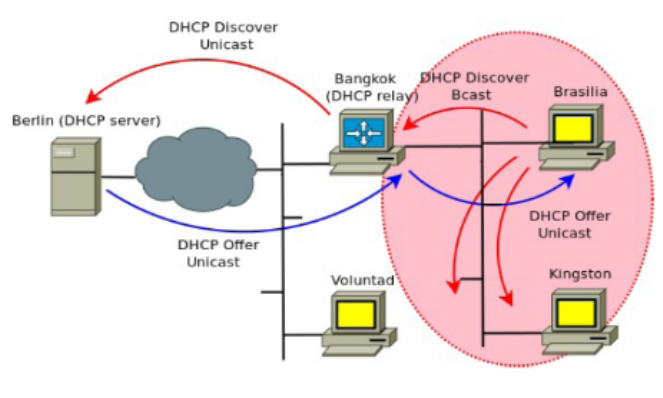
\includegraphics[width=0.5\textwidth]{capitulos/dhcp/imagenes/dhcp-relay.png}
    \caption{Ejemplo de DHCP Relay}
    \label{fig:dhcp-relay}
\end{figure}
